\documentclass[11pt,a4paper]{article}
\usepackage[spanish,es-nodecimaldot]{babel}	% Utilizar español
\usepackage[utf8]{inputenc}					% Caracteres UTF-8
\usepackage{graphicx}						% Imagenes
\usepackage[hidelinks]{hyperref}			% Poner enlaces sin marcarlos en rojo
\usepackage{fancyhdr}						% Modificar encabezados y pies de pagina
\usepackage{float}							% Insertar figuras
\usepackage[textwidth=390pt]{geometry}		% Anchura de la pagina
\usepackage[nottoc]{tocbibind}				% Referencias (no incluir num pagina indice en Indice)
\usepackage{enumitem}						% Permitir enumerate con distintos simbolos
\usepackage[T1]{fontenc}					% Usar textsc en sections
\usepackage{amsmath}						% Símbolos matemáticos
\usepackage{listings}
\usepackage{color}

 
\definecolor{codegreen}{rgb}{0,0.6,0}
\definecolor{codegray}{rgb}{0.5,0.5,0.5}
\definecolor{codepurple}{rgb}{0.58,0,0.82}
\definecolor{backcolour}{rgb}{0.99,0.99,0.99}
 
\lstdefinestyle{mystyle}{
    backgroundcolor=\color{backcolour},   
    commentstyle=\color{codegreen},
    keywordstyle=\color{magenta},
    numberstyle=\tiny\color{codegray},
    stringstyle=\color{codepurple},
    basicstyle=\footnotesize,
    breakatwhitespace=false,         
    breaklines=true,                 
    captionpos=b,                    
    keepspaces=true,                 
    numbers=left,                    
    numbersep=5pt,                  
    showspaces=false,                
    showstringspaces=false,
    showtabs=false,                  
    tabsize=2
}
 
\lstset{style=mystyle, language=Python}

% Comando para poner el nombre de la asignatura
\newcommand{\asignatura}{Inteligencia de Negocio}
\newcommand{\autor}{José María Sánchez Guerrero}
\newcommand{\titulo}{Práctica 1}
\newcommand{\subtitulo}{Resolución de problemas de clasificación y análisis experimental.}

% Configuracion de encabezados y pies de pagina
\pagestyle{fancy}
\lhead{\autor{}}
\rhead{\asignatura{}}
\lfoot{Grado en Ingeniería Informática}
\cfoot{}
\rfoot{\thepage}
\renewcommand{\headrulewidth}{0.4pt}		% Linea cabeza de pagina
\renewcommand{\footrulewidth}{0.4pt}		% Linea pie de pagina

\begin{document}
\pagenumbering{gobble}

% Pagina de titulo
\begin{titlepage}

\begin{minipage}{\textwidth}

\centering


\includegraphics[scale=0.5]{img/ugr.png}\\

\textsc{\Large \asignatura{}\\[0.2cm]}
\textsc{GRADO EN INGENIERÍA INFORMÁTICA}\\[1cm]

\noindent\rule[-1ex]{\textwidth}{1pt}\\[1.5ex]
\textsc{{\Huge \titulo\\[0.5ex]}}
\textsc{{\Large \subtitulo\\}}
\noindent\rule[-1ex]{\textwidth}{2pt}\\[3.5ex]

\end{minipage}

\vspace{0.5cm}

\begin{minipage}{\textwidth}

\centering

\textbf{Autor}\\ {\autor{}}\\[2.5ex]
\textbf{Rama}\\ {Computación y Sistemas Inteligentes}\\[2.5ex]
\vspace{0.3cm}


\includegraphics[scale=0.3]{img/etsiit.jpeg}

\vspace{0.3cm}
\textsc{Escuela Técnica Superior de Ingenierías Informática y de Telecomunicación}\\
\vspace{1cm}
\textsc{Curso 2020-2021}
\end{minipage}
\end{titlepage}

\pagenumbering{arabic}
\tableofcontents
\thispagestyle{empty}				% No usar estilo en la pagina de indice

\newpage

\setlength{\parskip}{1em}



\section{Introducción}

En este trabajo vamos a analizar el comportamiento de distintos algoritmos de clasificación en el problema propuesto. Disponemos
de un dataset, llamado \textit{''Mammographic Mass dataset''}, en el cual se desea predecir el tipo de tumor (benigno o maligno)
en una serie de mamografías realizadas para un estudio sobre el cáncer de mama. Este estudio lo vamos a realizar gracias a los
siguientes atributos proporcionados en el dataset:

\begin{itemize}
	\item \textbf{BI-RADS.} Este parámetro representa un control de calidad de las mamografías. Consta de 7 categorías distintas,
		  en las que, cuanto más alto sea el valor, hay una mayor probabilidad de que sea maligno.

	\item \textbf{Edad} del paciente.
	
	\item \textbf{Forma de la masa.} Dependiendo de como sea la masa anormal detectada, se clasifica como \textbf{R}edondeada,
		  \textbf{O}valada, \textbf{L}obulada, \textbf{I}rregular ó \textbf{N}o definida.

	\item \textbf{Margen de masa.} Circumscribed = 1, microlobulated = 2, obscured = 3, ill-defined = 4, spiculated = 5 (nominal).
	
	\item \textbf{Densidad de la masa.} Valores entre 1 y 4, siendo 1 la más alta y 4 contenido graso (no tumoral).
	
	\item \textbf{Severidad.} Es el atributo que se desea predecir, es decir, si es un tumor benigno o maligno.	

\end{itemize}

En el dataset hay datos de 961 pacientes, sin embargo, nos gustaría dejar un porcentaje para validar el modelo y así ver cómo va
entrenando los datos. Posteriormente, se explicará cómo se ha determinado qué datos son los de entrenamiento y cuáles son los de
test.

\newpage

\section{Procesado de datos}

Lo primero que tenemos que hacer es mostrar varios de los datos que tenemos y analizarlos. En mi caso vamos a sacar las 5 primeras
filas:

\begin{table}[H]
    \centering
    \resizebox{\textwidth}{!}{%
    \begin{tabular}{|c|c|c|c|c|c|c|}
    \hline
    \textbf{} & \textbf{BI-RADS} & \textbf{Age} & \textbf{Shape} & \textbf{Margin} & \textbf{Density} & \textbf{Severity} \\ \hline
    \textbf{0} & 5.0 & 67.0 & L & 5.0 & 3.0 & maligno \\ \hline
    \textbf{1} & 4.0 & 43.0 & R & 1.0 & NaN & maligno \\ \hline
    \textbf{2} & 5.0 & 58.0 & I & 5.0 & 3.0 & maligno \\ \hline
    \textbf{3} & 4.0 & 28.0 & R & 1.0 & 3.0 & benigno \\ \hline
    \textbf{4} & 5.0 & 74.0 & R & 5.0 & NaN & maligno \\ \hline
    \end{tabular}%
    }
\end{table}

Podemos observar que tenemos tanto datos numéricos, como datos categóricos, como ya comentamos en la introducción. También podemos
observar que tenemos varias celdas con datos erróneos o perdidos (representados con el valor $NaN$), por lo que será importante
procesarlos para que nuestros algoritmos funcionen correctamente. Primero veamos qué cantidad de estos datos nulos tenemos:

\begin{table}[H]
    \centering
    \begin{tabular}{|l|l|}
    \hline
    \multicolumn{1}{|c|}{\textbf{BI-RADS}} & 2 \\ \hline
    \textbf{Age} & 5 \\ \hline
    \textbf{Shape} & 0 \\ \hline
    \textbf{Margin} & 48 \\ \hline
    \textbf{Density} & 76 \\ \hline
    \textbf{Severity} & 0 \\ \hline
    \end{tabular}
\end{table}

Son una cantidad bastante alta de datos, en comparación con la cantidad de datos totales que tenemos. Por lo tanto, eliminar toda
las filas que contengan uno, puede dejarnos con muy pocos datos para entrenar y validar, y que el modelo sea más débil. No obstante,
el introducir datos para reemplazar uno faltante ha de realizarse con cuidado, ya que no son datos reales.

También tenemos que tener en cuenta cuál es la distribución de estos datos antes de trabajar con ellos. Es decir, tenemos que
asegurarnos de no sesgar nuestros datos si los eliminamos. Si hay algún tipo de correlación, tendríamos que intentar completarlos
de alguna forma. Para ello, vamos a generar una gráfica para cada uno de los atributos del $dataset$, en la que mostraremos la
cantidad de datos antes y después de eliminarlos, y asi ver cómo están distribuidos.

\newpage
Los resultados son los siguientes:

\begin{figure}[H]
\centering

\begin{minipage}{0.5\textwidth}
    \centering
    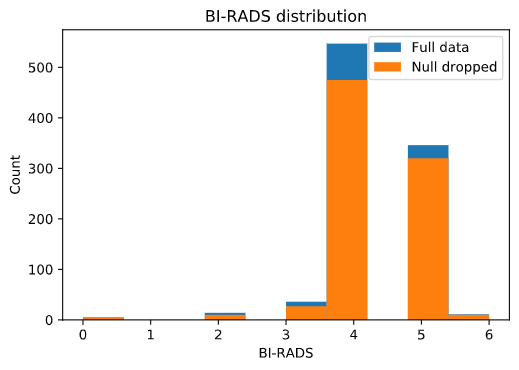
\includegraphics[scale=0.35]{img/birads-distribution.png}
\end{minipage}%
\begin{minipage}{0.5\textwidth}
    \centering
    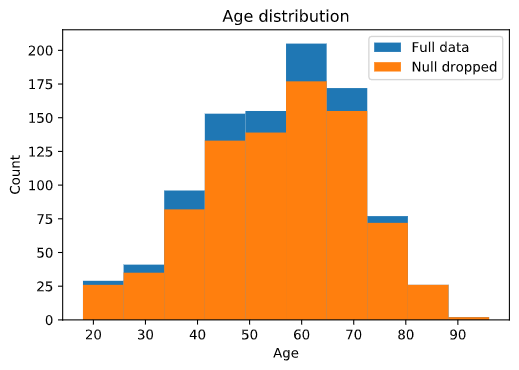
\includegraphics[scale=0.35]{img/age-distribution.png}
\end{minipage}

\end{figure}


\begin{figure}[H]
\centering

\begin{minipage}{0.5\textwidth}
    \centering
    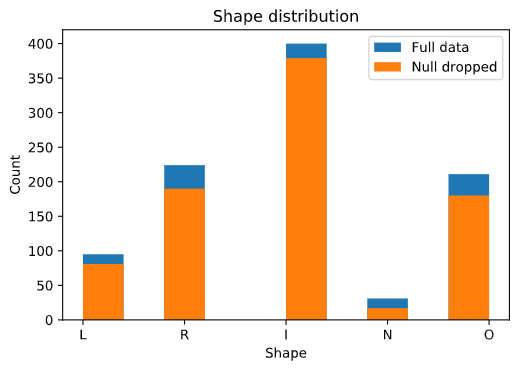
\includegraphics[scale=0.35]{img/shape-distribution.png}
\end{minipage}%
\begin{minipage}{0.5\textwidth}
    \centering
    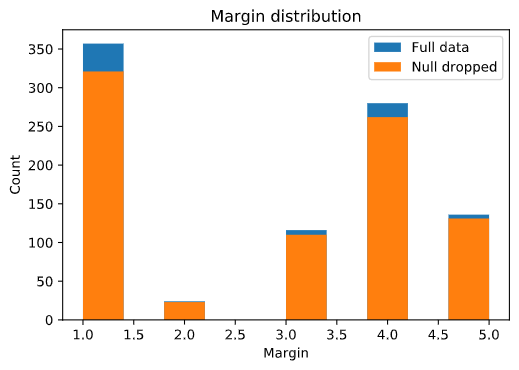
\includegraphics[scale=0.35]{img/margin-distribution.png}
\end{minipage}

\end{figure}


\begin{figure}[H]
\centering

\begin{minipage}{0.5\textwidth}
    \centering
    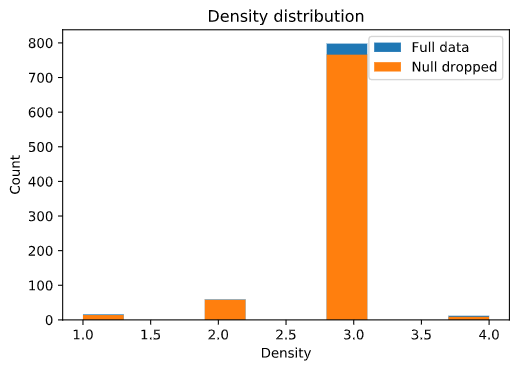
\includegraphics[scale=0.35]{img/density-distribution.png}
\end{minipage}%
\begin{minipage}{0.5\textwidth}
    \centering
    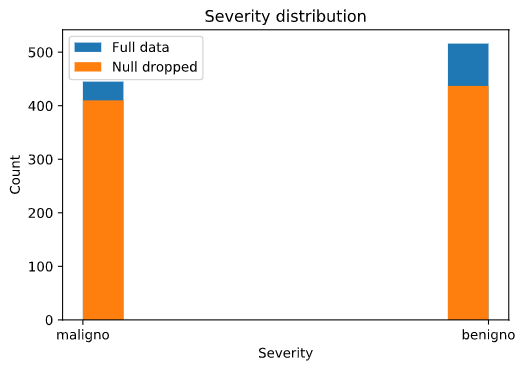
\includegraphics[scale=0.35]{img/severity-distribution.png}
\end{minipage}

\end{figure}

Podemos observar que los datos nulos están distribuidos aleatoriamente entre los atributos, por lo que podremos eliminarlos
del $dataset$ sin ningún problema (y teniendo en cuenta que tendremos menos datos para trabajar).

% PROBAR REEMPLAZANDO LOS DATOS CON ALEATORIOS
% \textit{Pandas} nos proporciona la función ''\textit{fillna()}'' para reemplazar los valores faltantes con un valor específico



\section{Configuración de algoritmos}
Para todos los algoritmos hemos procedido de la misma manera, y así evaluarlos a todos en igualdad de condiciones. Para
comenzar, declaramos el clasificador con sus parámetros correspondientes (en nuestro caso, las primeras evaluaciones han sido
con los parámetros por defecto y una semilla $random\_state=0$).

Posteriormente, hacemos las predicciones correspondientes para los datos de entrenamiento. Lo hacemos mediante validación
cruzada de 5 particiones, gracias a la función:
$$cross\_val\_predict(classifier, x\_train, y\_train, cv=5)$$

Por último, para evaluar los resultados obtenidos vamos a usar:
\begin{itemize}
    \item \textbf{Classification report.} Crea un informe que muestra las principales métricas de clasificación: precisión,
          recall, f1-score, y promedios macro, ponderado y de la muestra.
    \item \textbf{Score.} Misma medida del informe anterior mostrada con un poco más de precisión.
    \item \textbf{AUC Score.} Métrica que calcula el área bajo la curva ROC generada a partir de las predicciones.
    \item \textbf{Confusion matrix.} Muestra una matriz para evaluar la precisión de la clasificación. Cada fila representa las
          instancias de una clase predicha, mientras que cada columna representa las instancias reales de ésta.
\end{itemize}

Los algoritmos que evaluaremos han sido elegidos porque, cada uno de ellos, tiene una forma de procesar los datos diferente a
todos los demás. Estos algoritmos son los siguientes:

\subsection{K-Nearest-Neighbors (k-NN)}
Comenzamos por este algoritmo ya que es uno de los más utilizados, debido a su simplicidad. Este algoritmo funciona de la
siguiente manera. Cuando tenemos un nuevo ejemplo a clasificar, calcula la distancia (Euclídea) con respecto a los datos ya
existentes, y considerando los $k$ más cercanos, determina si pertenece a una clase u otra.

\newpage
A la hora de implementarlo lo hacemos de la siguiente forma:
$$KnnClf = KNeighborsClassifier(n\_neighbors=5)$$

Seleccionamos un número \textbf{k=5} de vecinos a evaluar y dejamos el resto de parámetros que trae el algoritmo por defecto.
El parámetro anterior es el más relevante, sin embargo, algunos otros interesantes a estudiar pueden ser, por ejemplo:
\textbf{p}, que sirve para cambiar el tipo de distancia utilizada (Euclídea, Manhattan o Minkowski); ó \textbf{weights}, que
determina la influencia de los vecinos en la predicción (todos ponderan igual, los cercanos influyen más o tu propia función).


\subsection*{Resultados obtenidos}
Hola buenas tardes


\subsection{Decision Tree}

\subsection*{Resultados obtenidos}


\subsection{Naive-Bayes}

\subsection*{Resultados obtenidos}


\subsection{Neural Network}

\subsection*{Resultados obtenidos}


\subsection{Support Vector Machine (SVM)}

\subsection*{Resultados obtenidos}


\section{Interpretación de los resultados}


\section{Conclusión}


\section{Bibliografía}


\end{document}